\documentclass[graphics]{beamer}
\usepackage{xcolor}
\usepackage{graphicx}
\usepackage{verbatim}
\usepackage{wrapfig}
\useoutertheme{shadow}
%\usecolortheme{orchid}
\usecolortheme{seahorse}


% math commands
\newcommand{\be}{\begin{eqnarray}}
\newcommand{\ee}{\end{eqnarray}}
\newcommand{\beq}{\begin{equation}}
\newcommand{\eeq}{\end{equation}}
\def\simless{\mathbin{\lower 3pt\hbox
      {$\rlap{\raise 5pt\hbox{$\char'074$}}\mathchar"7218$}}}
\def\simgreat{\mathbin{\lower 3pt\hbox
      {$\rlap{\raise 5pt\hbox{$\char'076$}}\mathchar"7218$}}} %> or of order

% variables

\def\toonscale{0.45}
\def\mboxy#1{\mbox{\small #1}}

\defbeamertemplate*{title page}{customized}[1][]
{
  \usebeamerfont{title}\inserttitle\par
  \usebeamerfont{subtitle}\usebeamercolor[fg]{subtitle}\insertsubtitle\par
  \bigskip
  \usebeamerfont{author}\insertauthor\par
  \usebeamerfont{institute}\insertinstitute\par
  \usebeamerfont{date}\insertdate\par
  \usebeamercolor[fg]{titlegraphic}\inserttitlegraphic
}
\begin{comment}
\AtBeginSection[]{
  \frame{
    \frametitle{Outline}
    \tableofcontents[currentsection]
  }
}
\end{comment}


\title{Interstellar Lenses}
%\subtitle{}
\author[U. Pen]{{
\textcolor{green}{\small Aladdin Seaifan, Dana Simard, Robert Main}, 
\textcolor{cyan}{\small I-Sheng Yang, Franz Kirsten} 
\textcolor{darkgray}{\small U. Pen, M. van Kerkwijk, K. Vanderlinde, J-P Macquart and many more}
}
\\[8mm] 
}
\date{May 11, 2016}


\begin{document}

\frame{
\vspace{-0.5in}
\begin{center}  
%\includegraphics[width=4.4in]{Figures/IMG-0438-by-Andre-cropped.jpg}
\end{center}
\begin{picture}(320,250)
\put(-50,60){
\includegraphics[width=5.5in]{Figures/traverse-aurora.jpg}}
\end{picture}
\vspace{-4in}
\\
image credit: Andre Recnik
\\
\vspace{1in}
\titlepage
}

%\section*{Introduction}
\section{Introduction}

\begin{comment}
  \subsection{Outline}

  \frame{
    \frametitle{Outline}
    \tableofcontents
  }
\end{comment}
  \frame{
    \frametitle{Pulsar Scintillometry}
    \begin{itemize}
        \item use interstellar plasma as billion km telescope
        \item unprecedented angular precision: 50 picoarcseconds, 6
          orders of magnitude improvement
    \item ULP+2014 picked up by 19 news outlets in 5 countries, over 26k youtube hits for Swinburne animation.
    \end{itemize}
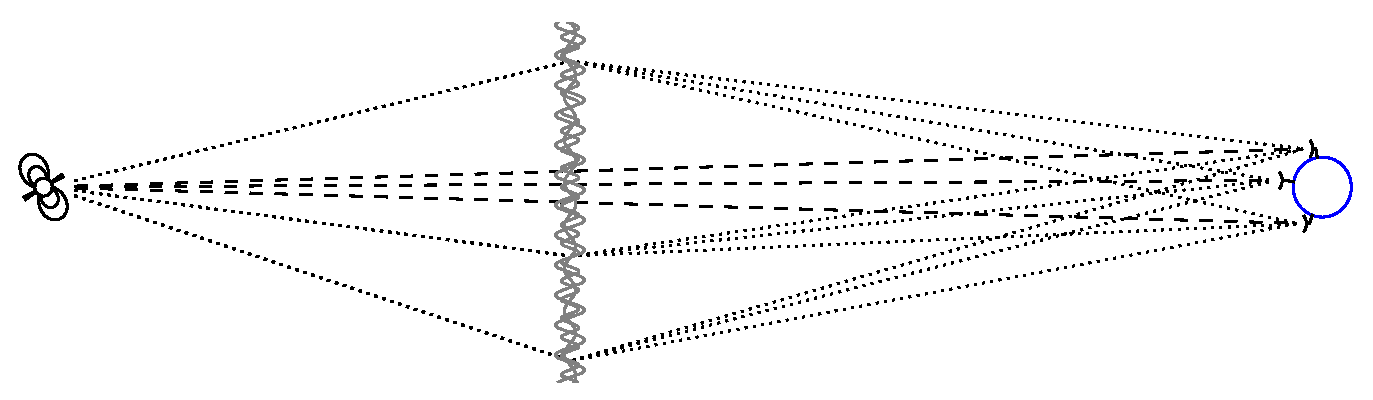
\includegraphics[width=4.5in]{Figures/scintillometry.eps}
}
  \frame{
    \frametitle{Scintellometry}
    \begin{itemize}
    \item Brisken et al 2010, ULP+2014  
    \end{itemize}
\hspace{-0.4in}\includegraphics[width=2.5in]{Figures/brisken.png}
\includegraphics[width=2.5in]{Figures/allgate.pdf}
}

  \frame{
    \frametitle{Plasma Lens Enigma}
    \begin{itemize}
        \item nature of lenses highly controversial
        \item observed bending angle requires extreme plasma conditions
        \item  exploding dark matter (Walker+2001), 
strange quark nuggets (Perez-Garcia+2014), 
superconducting cosmic strings
          (Thompson+2011), current sheets (UP+2014)
        \item distances, geometry, precisely measured
        \item treat like 'interstellar wormhole': make use of what's
          out there.
    \end{itemize}

  }


\section{Summary}
  \frame{
    \frametitle{Looking forward}
    \begin{itemize}
      \item regular DRAO-ARO broadband pulsar VLBI + other networks
      \item emission structure of pulsars
      \item binary orbit parameters: potentially most massive neutron
        star 1957+20?
      \item ISM lensing: precise distances?
      \item Pulsar size measurements, equation of state?
    \end{itemize}
  }


  \frame{
    \frametitle{Speculation}
    \begin{itemize}
    \item grazing incidence reconnection sheets
    \item ULP + Levin 2014
    \item ULP + King 2012
    \item Liu + ULP 2015
    \item 1-D structure
    \item localized scattering
%    \item predicts RM gradient
    \end{itemize}
\begin{picture}(320,235)
\put(110,170){
\includegraphics[width=3.0in]{Figures/toronto-skyline.png}}
\put(-60,-207){
\includegraphics[width=5.5in]{Figures/sheetgeom.eps}}
\end{picture}
  }
  \frame{
    \frametitle{Folds}
\begin{center}
\includegraphics[width=3.9in]{Figures/refraction.pdf}
\end{center}

Refraction of light rays near point D.  The black lines
  are the light paths.  The shaded region indicates the lensing sheet
  caustic.  The angles obey Snell's Law
  $\frac{\sin(\alpha_1)}{\sin(\alpha_2)}=\frac{\sin(\alpha_4)}{\sin(\alpha_3)}=\frac{n_{\rm sheet}}{n_{\rm
    ISM}.$ }
}

  \frame{
    \frametitle{Sheets}
\center{
\includegraphics[width=2.9in]{Figures/brisken.png}
}
}


  \frame{
    \frametitle{Conclusion}
    \begin{itemize}
      \item VLBI Scintillometry: cosmic lenses improve measurements by
        6 orders of magnitude
      \item Pulsar magnetosphere mapping: matter in extreme conditions
      \item ISM structure: mapping cosmic plasma and magnetic fields,
        unique probe on AU scales.
    \end{itemize}
  }

\end{document}
